%%=============================================================================
%% LaTeX sjabloon voor bachelorproef, HoGent Bedrijf en Organisatie
%% Opleiding Toegepaste Informatica
%%=============================================================================

\documentclass[fleqn,a4paper,12pt]{book}

%%=============================================================================
%% LaTeX sjabloon voor de bachelorproef, HoGent Bedrijf en Organisatie
%% Opleiding toegepaste informatica
%%
%% Structuur en algemene vormgeving. Meestal hoef je hier niets te wijzigen.
%%
%% Vormgeving gebaseerd op "The Legrand Orange Book", version 2.0 (9/2/15)
%% door Mathias Legrand (legrand.mathias@gmail.com) met aanpassingen door
%% Vel (vel@latextemplates.com). Het oorspronkelijke template is te vinden op
%% http://www.LaTeXTemplates.com
%%
%% Aanpassingen voor HoGent toegepaste informatica: 
%%   Bert Van Vreckem <bert.vanvreckem@hogent.be>
%% Licentie: 
%%   CC BY-NC-SA 3.0 (http://creativecommons.org/licenses/by-nc-sa/3.0/)
%%=============================================================================

%%-----------------------------------------------------------------------------
%% Packages
%%-----------------------------------------------------------------------------

\usepackage[top=3cm,bottom=3cm,left=3cm,right=3cm,headsep=10pt,a4paper]{geometry} % Page margins
\usepackage[utf8]{inputenc}  % Accenten gebruiken in tekst (vb. é ipv \'e)
\usepackage{amsfonts}        % AMS math packages: extra wiskundige
\usepackage{amsmath}         %   symbolen (o.a. getallen-
\usepackage{amssymb}         %   verzamelingen N, R, Z, Q, etc.)
\usepackage[english,dutch]{babel}    % Taalinstellingen: woordsplitsingen,
                             %  commando's voor speciale karakters
                             %  ("dutch" voor NL)
\usepackage{iflang}
\usepackage{eurosym}         % Euro-symbool €
\usepackage{geometry}
\usepackage{graphicx}        % Invoegen van tekeningen
\graphicspath{{img/}}       % Specifies the directory where pictures are stored
\usepackage{tikz}            % Required for drawing custom shapes
\usepackage[pdftex,bookmarks=true]{hyperref}
                             % PDF krijgt klikbare links & verwijzingen,
                             %  inhoudstafel
\usepackage{enumitem}        % Customize lists
\setlist{nolistsep}         % Reduce spacing between list items
\usepackage{listings}        % Broncode mooi opmaken
\usepackage{multirow}        % Tekst over verschillende cellen in tabellen
\usepackage{rotating}        % Tabellen en figuren roteren

\usepackage{booktabs}        % Required for nicer horizontal rules in tables

\usepackage{xcolor}          % Required for specifying colors by name
\definecolor{maincolor}{RGB}{0,147,208} % Define the main color used for 
                             % highlighting throughout the book
                             % 0, 147, 208 = officiële kleur HoGent FBO

% Paragraph style: no indent, add space between paragraphs
\setlength{\parindent}{0em}
\setlength{\parskip}{1em}

\usepackage{etoolbox}
\usepackage{titling} % Macros for title, author, etc
\usepackage{lipsum}          % Voor vultekst (lorem ipsum)

%----------------------------------------------------------------------------------------
%	FONTS
%----------------------------------------------------------------------------------------

\usepackage{avant} % Use the Avantgarde font for headings
%\usepackage{times} % Use the Times font for headings
\usepackage{mathptmx} % Use the Adobe Times Roman as the default text font together with math symbols from the Sym­bol, Chancery and Com­puter Modern fonts

\usepackage{microtype} % Slightly tweak font spacing for aesthetics
\usepackage[utf8]{inputenc} % Required for including letters with accents
\usepackage[T1]{fontenc} % Use 8-bit encoding that has 256 glyphs

%------------------------------------------------------------------------------
%	TITLE PAGE
%------------------------------------------------------------------------------

\newcommand{\inserttitlepage}{%
\begin{titlepage}
  \newgeometry{top=2cm,bottom=1.5cm,left=1.5cm,right=1.5cm}
  \begin{center}

    \begingroup
    \rmfamily
    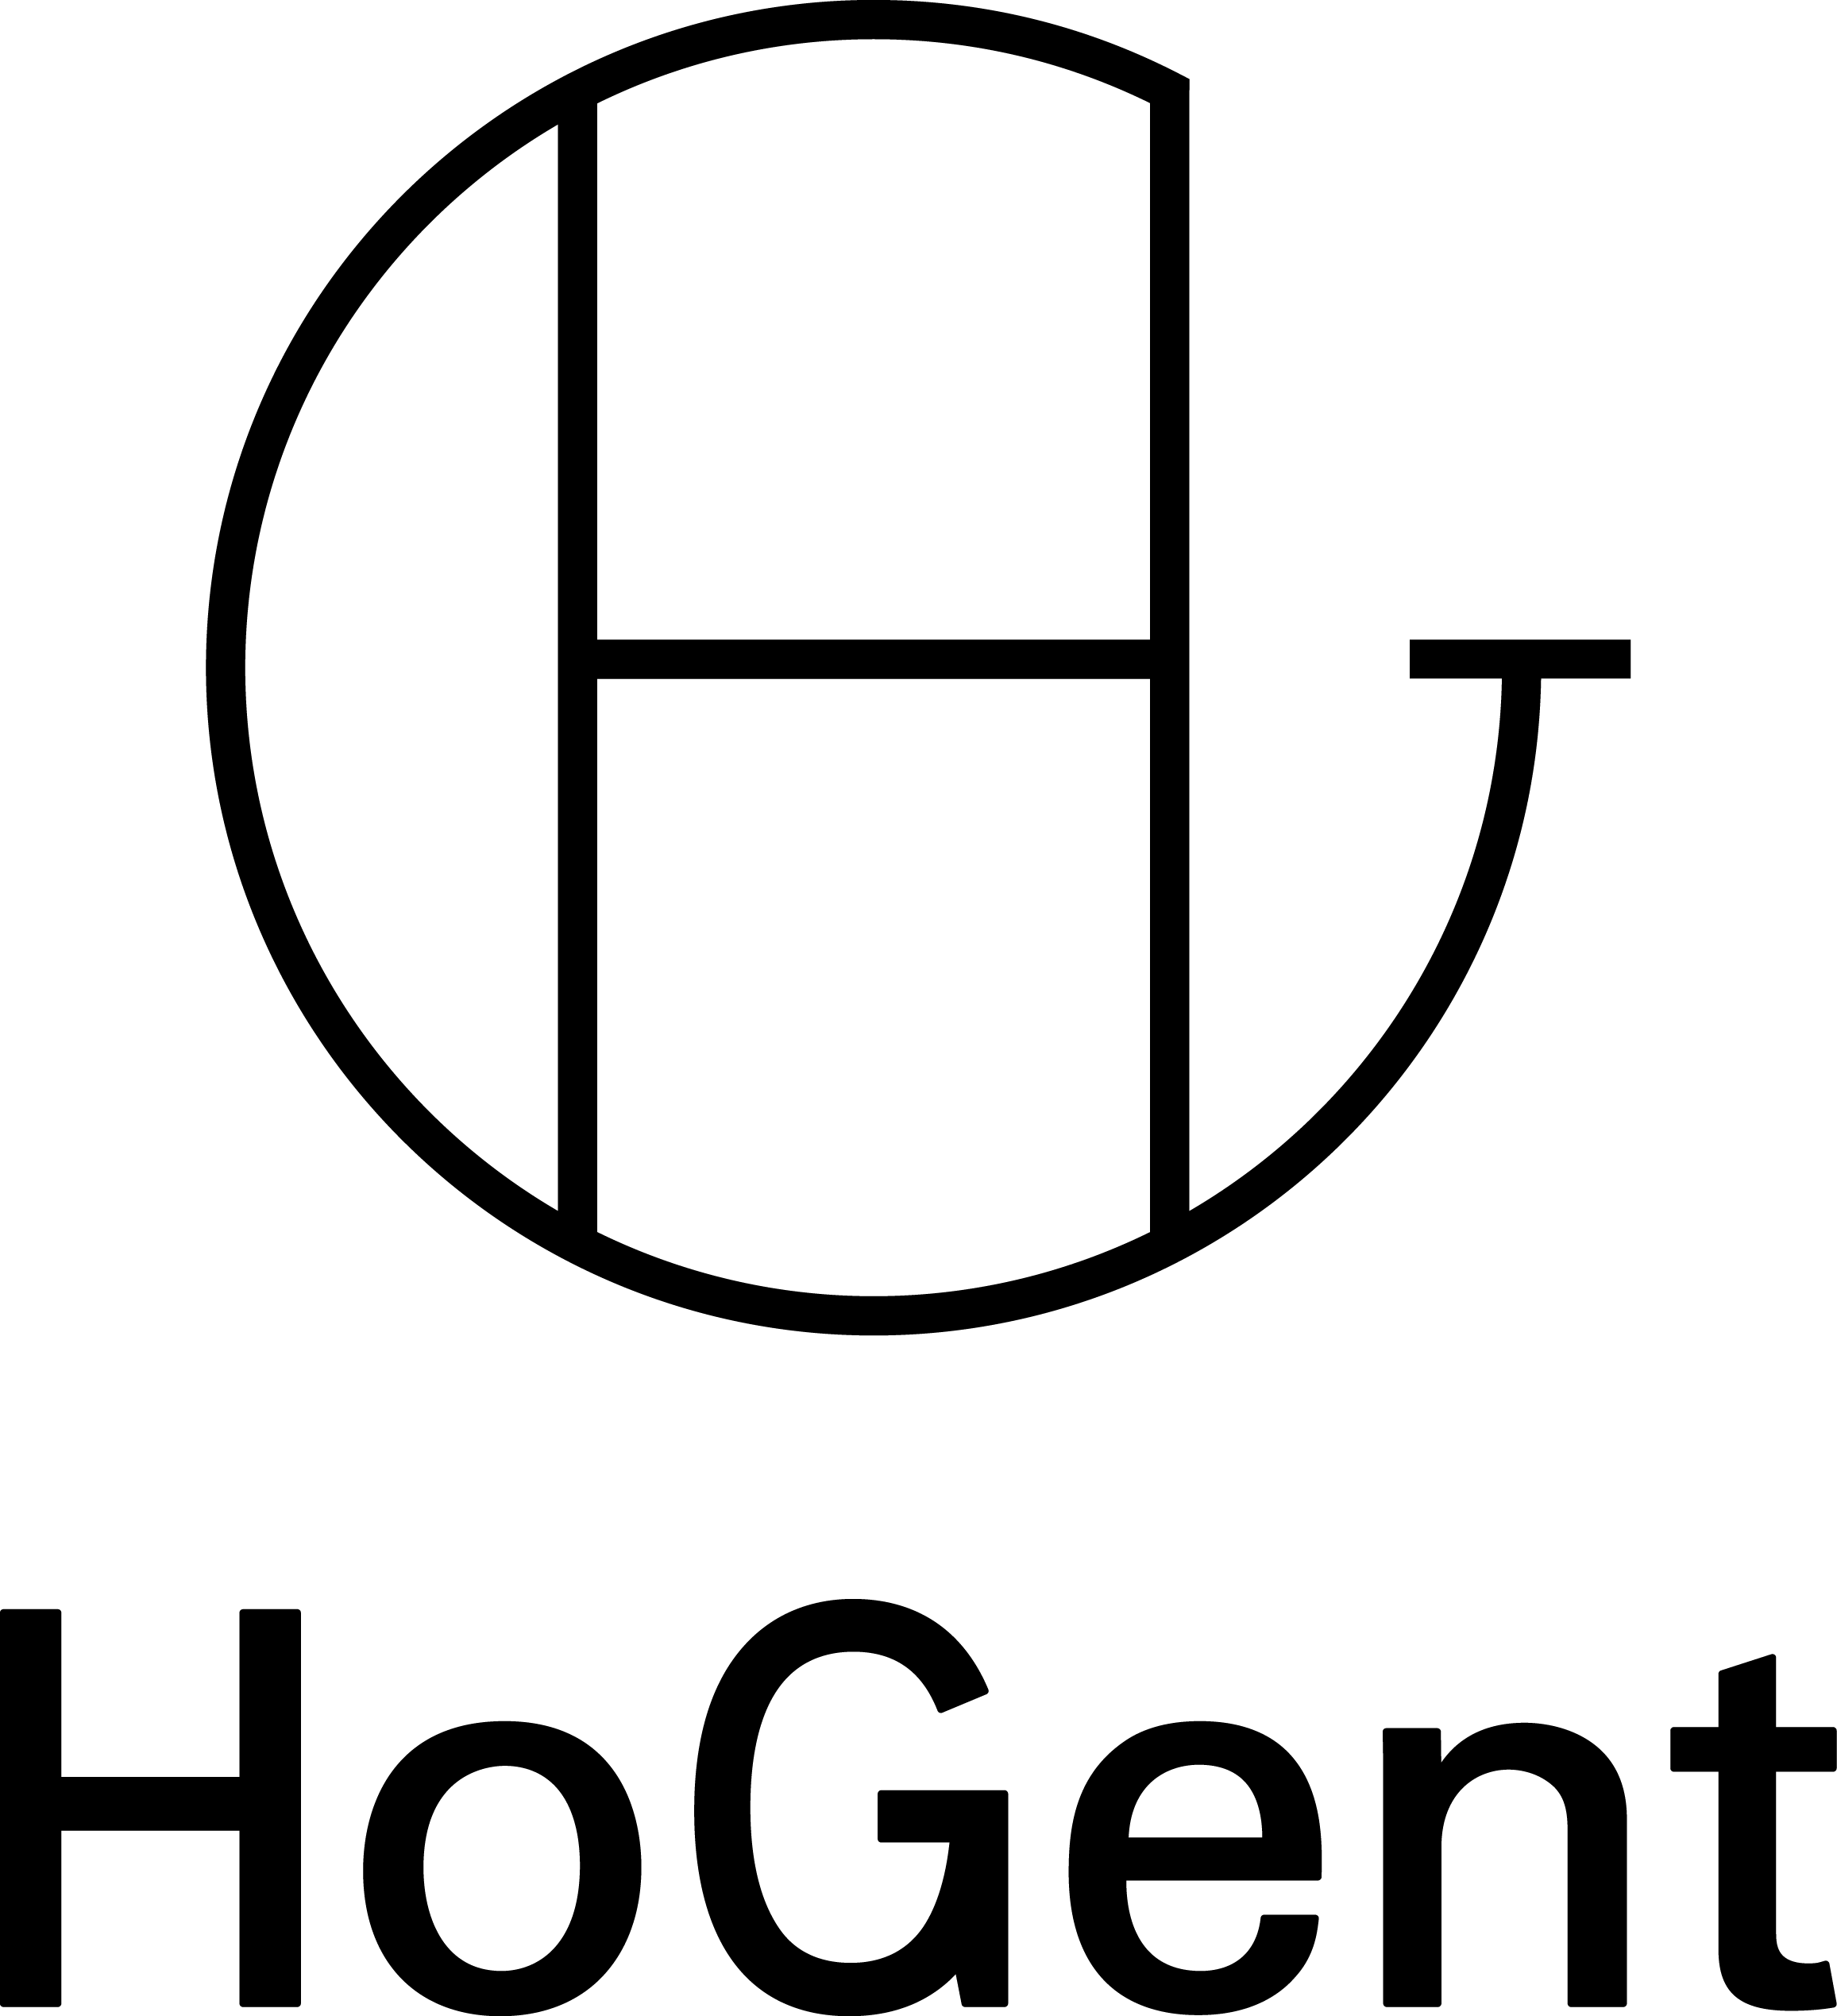
\includegraphics[width=2.5cm]{img/HG-beeldmerk-woordmerk}\\[.5cm]
    Faculteit Bedrijf en Organisatie\\[3cm]
    \titel
    \vfill
    \student\\[3.5cm]
    Scriptie voorgedragen tot het bekomen van de graad van\\professionele bachelor in de toegepaste informatica\\[2cm]
    Promotor:\\
    \promotor\\
    \ifdefempty{\copromotor}{\vspace{2.5cm}}{Co-promotor:\\\copromotor\\[2.5cm]}
    Instelling: \instelling\\[.5cm]
    Academiejaar: \academiejaar\\[.5cm]
    \ifcase \examenperiode \or Eerste \or Tweede \else Derde \fi examenperiode
    \endgroup

  \end{center}
  \restoregeometry
\end{titlepage}
  \emptypage
\begin{titlepage}
  \newgeometry{top=5.35cm,bottom=1.5cm,left=1.5cm,right=1.5cm}
  \begin{center}

    \begingroup
    \rmfamily
    \IfLanguageName{dutch}{Faculteit Bedrijf en Organisatie}{Faculty of Business and Information Management}\\[3cm]
    \titel
    \vfill
    \student\\[3.5cm]
    \IfLanguageName{dutch}{Scriptie voorgedragen tot het bekomen van de graad van\\professionele bachelor in de toegepaste informatica}{Thesis submitted in partial fulfilment of the requirements for the degree of\\professional bachelor of applied computer science}\\[2cm]
    Promotor:\\
    \promotor\\
    \ifdefempty{\copromotor}{\vspace{2.5cm}}{Co-promotor:\\\copromotor\\[2.5cm]}
    \IfLanguageName{dutch}{Instelling}{Institution}: \instelling\\[.5cm]
    \IfLanguageName{dutch}{Academiejaar}{Academic year}: \academiejaar\\[.5cm]
    \IfLanguageName{dutch}{%
    \ifcase \examenperiode \or Eerste \or Tweede \else Derde \fi examenperiode}{%
    \ifcase \examenperiode \or First \or Second \else Third \fi examination period}
    \endgroup

  \end{center}
  \restoregeometry
\end{titlepage}
}

%----------------------------------------------------------------------------------------
%	BIBLIOGRAPHY AND INDEX
%----------------------------------------------------------------------------------------

\usepackage[style=apa,backend=biber]{biblatex}
\usepackage{csquotes}
\DeclareLanguageMapping{dutch}{dutch-apa}
\addbibresource{bachproef-tin.bib} % BibTeX bibliography file
\defbibheading{bibempty}{}

\usepackage{calc} % For simpler calculation - used for spacing the index letter headings correctly
\usepackage{makeidx} % Required to make an index
\makeindex % Tells LaTeX to create the files required for indexing

%----------------------------------------------------------------------------------------
%	MAIN TABLE OF CONTENTS
%----------------------------------------------------------------------------------------

\usepackage{titletoc} % Required for manipulating the table of contents

\contentsmargin{0cm} % Removes the default margin

% Part text styling
\titlecontents{part}[0cm]
{\addvspace{20pt}\centering\large\bfseries}
{}
{}
{}

% Chapter text styling
\titlecontents{chapter}[1.25cm] % Indentation
{\addvspace{12pt}\large\sffamily\bfseries} % Spacing and font options for chapters
{\color{maincolor!60}\contentslabel[\Large\thecontentslabel]{1.25cm}\color{maincolor}} % Chapter number
{\color{maincolor}}
{\color{maincolor!60}\normalsize\;\titlerule*[.5pc]{.}\;\thecontentspage} % Page number

% Section text styling
\titlecontents{section}[1.25cm] % Indentation
{\addvspace{3pt}\sffamily\bfseries} % Spacing and font options for sections
{\contentslabel[\thecontentslabel]{1.25cm}} % Section number
{}
{\hfill\color{black}\thecontentspage} % Page number
[]

% Subsection text styling
\titlecontents{subsection}[1.25cm] % Indentation
{\addvspace{1pt}\sffamily\small} % Spacing and font options for subsections
{\contentslabel[\thecontentslabel]{1.25cm}} % Subsection number
{}
{\ \titlerule*[.5pc]{.}\;\thecontentspage} % Page number
[]

% List of figures
\titlecontents{figure}[0em]
{\addvspace{-5pt}\sffamily}
{\thecontentslabel\hspace*{1em}}
{}
{\ \titlerule*[.5pc]{.}\;\thecontentspage}
[]

% List of tables
\titlecontents{table}[0em]
{\addvspace{-5pt}\sffamily}
{\thecontentslabel\hspace*{1em}}
{}
{\ \titlerule*[.5pc]{.}\;\thecontentspage}
[]

%----------------------------------------------------------------------------------------
%	MINI TABLE OF CONTENTS IN PART HEADS
%----------------------------------------------------------------------------------------

% Chapter text styling
\titlecontents{lchapter}[0em] % Indenting
{\addvspace{15pt}\large\sffamily\bfseries} % Spacing and font options for chapters
{\color{maincolor}\contentslabel[\Large\thecontentslabel]{1.25cm}\color{maincolor}} % Chapter number
{}
{\color{maincolor}\normalsize\sffamily\bfseries\;\titlerule*[.5pc]{.}\;\thecontentspage} % Page number

% Section text styling
\titlecontents{lsection}[0em] % Indenting
{\sffamily\small} % Spacing and font options for sections
{\contentslabel[\thecontentslabel]{1.25cm}} % Section number
{}
{}

% Subsection text styling
\titlecontents{lsubsection}[.5em] % Indentation
{\normalfont\footnotesize\sffamily} % Font settings
{}
{}
{}

%----------------------------------------------------------------------------------------
%	PAGE HEADERS
%----------------------------------------------------------------------------------------

\usepackage{fancyhdr} % Required for header and footer configuration

\pagestyle{fancy}
\renewcommand{\chaptermark}[1]{\markboth{\sffamily\normalsize\bfseries\chaptername\ \thechapter.\ #1}{}} % Chapter text font settings
\renewcommand{\sectionmark}[1]{\markright{\sffamily\normalsize\thesection\hspace{5pt}#1}{}} % Section text font settings
\fancyhf{} \fancyhead[LE,RO]{\sffamily\normalsize\thepage} % Font setting for the page number in the header
\fancyhead[LO]{\rightmark} % Print the nearest section name on the left side of odd pages
\fancyhead[RE]{\leftmark} % Print the current chapter name on the right side of even pages
\renewcommand{\headrulewidth}{0.5pt} % Width of the rule under the header
\addtolength{\headheight}{2.5pt} % Increase the spacing around the header slightly
\renewcommand{\footrulewidth}{0pt} % Removes the rule in the footer
\fancypagestyle{plain}{\fancyhead{}\renewcommand{\headrulewidth}{0pt}} % Style for when a plain pagestyle is specified

% Removes the header from odd empty pages at the end of chapters
\makeatletter
\renewcommand{\cleardoublepage}{
\clearpage\ifodd\c@page\else
\hbox{}
\vspace*{\fill}
\thispagestyle{empty}
\newpage
\fi}

%----------------------------------------------------------------------------------------
%	THEOREM STYLES
%----------------------------------------------------------------------------------------

\usepackage{amsmath,amsfonts,amssymb,amsthm} % For math equations, theorems, symbols, etc

\newcommand{\intoo}[2]{\mathopen{]}#1\,;#2\mathclose{[}}
\newcommand{\ud}{\mathop{\mathrm{{}d}}\mathopen{}}
\newcommand{\intff}[2]{\mathopen{[}#1\,;#2\mathclose{]}}
\newtheorem{notation}{Notation}[chapter]

% Boxed/framed environments
\newtheoremstyle{maincolornumbox}% % Theorem style name
{0pt}% Space above
{0pt}% Space below
{\normalfont}% % Body font
{}% Indent amount
{\small\bf\sffamily\color{maincolor}}% % Theorem head font
{\;}% Punctuation after theorem head
{0.25em}% Space after theorem head
{\small\sffamily\color{maincolor}\thmname{#1}\nobreakspace\thmnumber{\@ifnotempty{#1}{}\@upn{#2}}% Theorem text (e.g. Theorem 2.1)
\thmnote{\nobreakspace\the\thm@notefont\sffamily\bfseries\color{black}---\nobreakspace#3.}} % Optional theorem note
\renewcommand{\qedsymbol}{$\blacksquare$}% Optional qed square

\newtheoremstyle{blacknumex}% Theorem style name
{5pt}% Space above
{5pt}% Space below
{\normalfont}% Body font
{} % Indent amount
{\small\bf\sffamily}% Theorem head font
{\;}% Punctuation after theorem head
{0.25em}% Space after theorem head
{\small\sffamily{\tiny\ensuremath{\blacksquare}}\nobreakspace\thmname{#1}\nobreakspace\thmnumber{\@ifnotempty{#1}{}\@upn{#2}}% Theorem text (e.g. Theorem 2.1)
\thmnote{\nobreakspace\the\thm@notefont\sffamily\bfseries---\nobreakspace#3.}}% Optional theorem note

\newtheoremstyle{blacknumbox} % Theorem style name
{0pt}% Space above
{0pt}% Space below
{\normalfont}% Body font
{}% Indent amount
{\small\bf\sffamily}% Theorem head font
{\;}% Punctuation after theorem head
{0.25em}% Space after theorem head
{\small\sffamily\thmname{#1}\nobreakspace\thmnumber{\@ifnotempty{#1}{}\@upn{#2}}% Theorem text (e.g. Theorem 2.1)
\thmnote{\nobreakspace\the\thm@notefont\sffamily\bfseries---\nobreakspace#3.}}% Optional theorem note

% Non-boxed/non-framed environments
\newtheoremstyle{maincolornum}% % Theorem style name
{5pt}% Space above
{5pt}% Space below
{\normalfont}% % Body font
{}% Indent amount
{\small\bf\sffamily\color{maincolor}}% % Theorem head font
{\;}% Punctuation after theorem head
{0.25em}% Space after theorem head
{\small\sffamily\color{maincolor}\thmname{#1}\nobreakspace\thmnumber{\@ifnotempty{#1}{}\@upn{#2}}% Theorem text (e.g. Theorem 2.1)
\thmnote{\nobreakspace\the\thm@notefont\sffamily\bfseries\color{black}---\nobreakspace#3.}} % Optional theorem note
\renewcommand{\qedsymbol}{$\blacksquare$}% Optional qed square
\makeatother

% Defines the theorem text style for each type of theorem to one of the three styles above
\newcounter{dummy}
\numberwithin{dummy}{section}
\theoremstyle{maincolornumbox}
\newtheorem{theoremeT}[dummy]{Theorem}
\newtheorem{problem}{Problem}[chapter]
\newtheorem{exerciseT}{Exercise}[chapter]
\theoremstyle{blacknumex}
\newtheorem{exampleT}{Example}[chapter]
\theoremstyle{blacknumbox}
\newtheorem{vocabulary}{Vocabulary}[chapter]
\newtheorem{definitionT}{Definition}[section]
\newtheorem{corollaryT}[dummy]{Corollary}
\theoremstyle{maincolornum}
\newtheorem{proposition}[dummy]{Proposition}

%----------------------------------------------------------------------------------------
%	DEFINITION OF COLORED BOXES
%----------------------------------------------------------------------------------------

\RequirePackage[framemethod=default]{mdframed} % Required for creating the theorem, definition, exercise and corollary boxes

% Theorem box
\newmdenv[skipabove=7pt,
skipbelow=7pt,
backgroundcolor=black!5,
linecolor=maincolor,
innerleftmargin=5pt,
innerrightmargin=5pt,
innertopmargin=5pt,
leftmargin=0cm,
rightmargin=0cm,
innerbottommargin=5pt]{tBox}

% Exercise box
\newmdenv[skipabove=7pt,
skipbelow=7pt,
rightline=false,
leftline=true,
topline=false,
bottomline=false,
backgroundcolor=maincolor!10,
linecolor=maincolor,
innerleftmargin=5pt,
innerrightmargin=5pt,
innertopmargin=5pt,
innerbottommargin=5pt,
leftmargin=0cm,
rightmargin=0cm,
linewidth=4pt]{eBox}

% Definition box
\newmdenv[skipabove=7pt,
skipbelow=7pt,
rightline=false,
leftline=true,
topline=false,
bottomline=false,
linecolor=maincolor,
innerleftmargin=5pt,
innerrightmargin=5pt,
innertopmargin=0pt,
leftmargin=0cm,
rightmargin=0cm,
linewidth=4pt,
innerbottommargin=0pt]{dBox}

% Corollary box
\newmdenv[skipabove=7pt,
skipbelow=7pt,
rightline=false,
leftline=true,
topline=false,
bottomline=false,
linecolor=gray,
backgroundcolor=black!5,
innerleftmargin=5pt,
innerrightmargin=5pt,
innertopmargin=5pt,
leftmargin=0cm,
rightmargin=0cm,
linewidth=4pt,
innerbottommargin=5pt]{cBox}

% Creates an environment for each type of theorem and assigns it a theorem text style from the "Theorem Styles" section above and a colored box from above
\newenvironment{theorem}{\begin{tBox}\begin{theoremeT}}{\end{theoremeT}\end{tBox}}
\newenvironment{exercise}{\begin{eBox}\begin{exerciseT}}{\hfill{\color{maincolor}\tiny\ensuremath{\blacksquare}}\end{exerciseT}\end{eBox}}
\newenvironment{definition}{\begin{dBox}\begin{definitionT}}{\end{definitionT}\end{dBox}}
\newenvironment{example}{\begin{exampleT}}{\hfill{\tiny\ensuremath{\blacksquare}}\end{exampleT}}
\newenvironment{corollary}{\begin{cBox}\begin{corollaryT}}{\end{corollaryT}\end{cBox}}

%----------------------------------------------------------------------------------------
%	REMARK ENVIRONMENT
%----------------------------------------------------------------------------------------

\newenvironment{remark}{\par\vspace{10pt}\small % Vertical white space above the remark and smaller font size
\begin{list}{}{
\leftmargin=35pt % Indentation on the left
\rightmargin=25pt}\item\ignorespaces % Indentation on the right
\makebox[-2.5pt]{\begin{tikzpicture}[overlay]
\node[draw=maincolor!60,line width=1pt,circle,fill=maincolor!25,font=\sffamily\bfseries,inner sep=2pt,outer sep=0pt] at (-15pt,0pt){\textcolor{maincolor}{R}};\end{tikzpicture}} % Orange R in a circle
\advance\baselineskip -1pt}{\end{list}\vskip5pt} % Tighter line spacing and white space after remark

%----------------------------------------------------------------------------------------
%	SECTION NUMBERING IN THE MARGIN
%----------------------------------------------------------------------------------------

\makeatletter
\renewcommand{\@seccntformat}[1]{\llap{\textcolor{maincolor}{\csname the#1\endcsname}\hspace{1em}}}
\renewcommand{\section}{\@startsection{section}{1}{\z@}
{-4ex \@plus -1ex \@minus -.4ex}
{1ex \@plus.2ex }
{\normalfont\large\sffamily\bfseries}}
\renewcommand{\subsection}{\@startsection {subsection}{2}{\z@}
{-3ex \@plus -0.1ex \@minus -.4ex}
{0.5ex \@plus.2ex }
{\normalfont\sffamily\bfseries}}
\renewcommand{\subsubsection}{\@startsection {subsubsection}{3}{\z@}
{-2ex \@plus -0.1ex \@minus -.2ex}
{.2ex \@plus.2ex }
{\normalfont\small\sffamily\bfseries}}
\renewcommand\paragraph{\@startsection{paragraph}{4}{\z@}
{-2ex \@plus-.2ex \@minus .2ex}
{.1ex}
{\normalfont\small\sffamily\bfseries}}

%----------------------------------------------------------------------------------------
%	PART HEADINGS
%----------------------------------------------------------------------------------------

% numbered part in the table of contents
\newcommand{\@mypartnumtocformat}[2]{%
\setlength\fboxsep{0pt}%
\noindent\colorbox{maincolor!20}{\strut\parbox[c][.7cm]{\ecart}{\color{maincolor!70}\Large\sffamily\bfseries\centering#1}}\hskip\esp\colorbox{maincolor!40}{\strut\parbox[c][.7cm]{\linewidth-\ecart-\esp}{\Large\sffamily\centering#2}}}%
%%%%%%%%%%%%%%%%%%%%%%%%%%%%%%%%%%
% unnumbered part in the table of contents
\newcommand{\@myparttocformat}[1]{%
\setlength\fboxsep{0pt}%
\noindent\colorbox{maincolor!40}{\strut\parbox[c][.7cm]{\linewidth}{\Large\sffamily\centering#1}}}%
%%%%%%%%%%%%%%%%%%%%%%%%%%%%%%%%%%
\newlength\esp
\setlength\esp{4pt}
\newlength\ecart
\setlength\ecart{1.2cm-\esp}
\newcommand{\thepartimage}{}%
\newcommand{\partimage}[1]{\renewcommand{\thepartimage}{#1}}%
\def\@part[#1]#2{%
\ifnum \c@secnumdepth >-2\relax%
\refstepcounter{part}%
\addcontentsline{toc}{part}{\texorpdfstring{\protect\@mypartnumtocformat{\thepart}{#1}}{\partname~\thepart\ ---\ #1}}
\else%
\addcontentsline{toc}{part}{\texorpdfstring{\protect\@myparttocformat{#1}}{#1}}%
\fi%
\startcontents%
\markboth{}{}%
{\thispagestyle{empty}%
\begin{tikzpicture}[remember picture,overlay]%
\node at (current page.north west){\begin{tikzpicture}[remember picture,overlay]%
\fill[maincolor!20](0cm,0cm) rectangle (\paperwidth,-\paperheight);
\node[anchor=north] at (4cm,-3.25cm){\color{maincolor!40}\fontsize{220}{100}\sffamily\bfseries\@Roman\c@part};
\node[anchor=south east] at (\paperwidth-1cm,-\paperheight+1cm){\parbox[t][][t]{8.5cm}{
\printcontents{l}{0}{\setcounter{tocdepth}{1}}%
}};
\node[anchor=north east] at (\paperwidth-1.5cm,-3.25cm){\parbox[t][][t]{15cm}{\strut\raggedleft\color{white}\fontsize{30}{30}\sffamily\bfseries#2}};
\end{tikzpicture}};
\end{tikzpicture}}%
\@endpart}
\def\@spart#1{%
\startcontents%
\phantomsection
{\thispagestyle{empty}%
\begin{tikzpicture}[remember picture,overlay]%
\node at (current page.north west){\begin{tikzpicture}[remember picture,overlay]%
\fill[maincolor!20](0cm,0cm) rectangle (\paperwidth,-\paperheight);
\node[anchor=north east] at (\paperwidth-1.5cm,-3.25cm){\parbox[t][][t]{15cm}{\strut\raggedleft\color{white}\fontsize{30}{30}\sffamily\bfseries#1}};
\end{tikzpicture}};
\end{tikzpicture}}
\addcontentsline{toc}{part}{\texorpdfstring{%
\setlength\fboxsep{0pt}%
\noindent\protect\colorbox{maincolor!40}{\strut\protect\parbox[c][.7cm]{\linewidth}{\Large\sffamily\protect\centering #1\quad\mbox{}}}}{#1}}%
\@endpart}
\def\@endpart{\vfil\newpage
\if@twoside
\if@openright
\null
\thispagestyle{empty}%
\newpage
\fi
\fi
\if@tempswa
\twocolumn
\fi}

%----------------------------------------------------------------------------------------
%	CHAPTER HEADINGS
%----------------------------------------------------------------------------------------

% A switch to conditionally include a picture, implemented by  Christian Hupfer
\newif\ifusechapterimage
\usechapterimagetrue
\newcommand{\thechapterimage}{}%
\newcommand{\chapterimage}[1]{\ifusechapterimage\renewcommand{\thechapterimage}{#1}\fi}%
\def\@makechapterhead#1{%
{\parindent \z@ \raggedright \normalfont
\ifnum \c@secnumdepth >\m@ne
\if@mainmatter
\begin{tikzpicture}[remember picture,overlay]
\node at (current page.north west)
{\begin{tikzpicture}[remember picture,overlay]
\node[anchor=north west,inner sep=0pt] at (0,0) {\ifusechapterimage\includegraphics[width=\paperwidth]{\thechapterimage}\fi};
\draw[anchor=west] (\Gm@lmargin,-9cm) node [line width=2pt,rounded corners=15pt,draw=maincolor,fill=white,fill opacity=0.5,inner sep=15pt]{\strut\makebox[22cm]{}};
\draw[anchor=west] (\Gm@lmargin+.3cm,-9cm) node {\huge\sffamily\bfseries\color{black}\thechapter. #1\strut};
\end{tikzpicture}};
\end{tikzpicture}
\else
\begin{tikzpicture}[remember picture,overlay]
\node at (current page.north west)
{\begin{tikzpicture}[remember picture,overlay]
\node[anchor=north west,inner sep=0pt] at (0,0) {\ifusechapterimage\includegraphics[width=\paperwidth]{\thechapterimage}\fi};
\draw[anchor=west] (\Gm@lmargin,-9cm) node [line width=2pt,rounded corners=15pt,draw=maincolor,fill=white,fill opacity=0.5,inner sep=15pt]{\strut\makebox[22cm]{}};
\draw[anchor=west] (\Gm@lmargin+.3cm,-9cm) node {\huge\sffamily\bfseries\color{black}#1\strut};
\end{tikzpicture}};
\end{tikzpicture}
\fi\fi\par\vspace*{270\p@}}}

%-------------------------------------------

\def\@makeschapterhead#1{%
\begin{tikzpicture}[remember picture,overlay]
\node at (current page.north west)
{\begin{tikzpicture}[remember picture,overlay]
\node[anchor=north west,inner sep=0pt] at (0,0) {\ifusechapterimage\includegraphics[width=\paperwidth]{\thechapterimage}\fi};
\draw[anchor=west] (\Gm@lmargin,-9cm) node [line width=2pt,rounded corners=15pt,draw=maincolor,fill=white,fill opacity=0.5,inner sep=15pt]{\strut\makebox[22cm]{}};
\draw[anchor=west] (\Gm@lmargin+.3cm,-9cm) node {\huge\sffamily\bfseries\color{black}#1\strut};
\end{tikzpicture}};
\end{tikzpicture}
\par\vspace*{270\p@}}
\makeatother

%----------------------------------------------------------------------------------------
%	HYPERLINKS IN THE DOCUMENTS
%----------------------------------------------------------------------------------------

\usepackage{hyperref}
\hypersetup{hidelinks,backref=true,pagebackref=true,hyperindex=true,colorlinks=false,breaklinks=true,urlcolor= maincolor,bookmarks=true,bookmarksopen=false,pdftitle={Title},pdfauthor={Author}}
\usepackage{bookmark}
\bookmarksetup{
open,
numbered,
addtohook={%
\ifnum\bookmarkget{level}=0 % chapter
\bookmarksetup{bold}%
\fi
\ifnum\bookmarkget{level}=-1 % part
\bookmarksetup{color=maincolor,bold}%
\fi
}
}

%----------------------------------------------------------------------------------------
%	Java source code
%----------------------------------------------------------------------------------------

% Commando voor invoegen Java-broncodebestanden (dank aan Niels Corneille)
% Gebruik:
%   \codefragment{source/MijnKlasse.java}{Uitleg bij de code}
%
% Je kan dit aanpassen aan de taal die je zelf het meeste gebruikt in je
% bachelorproef.
\newcommand{\codefragment}[2]{ \lstset{%
  language=java,
  breaklines=true,
  float=th,
  caption={#2},
  basicstyle=\scriptsize,
  frame=single,
  extendedchars=\true
}
\lstinputlisting{#1}}

% Leeg blad
\newcommand{\emptypage}{%
\newpage
\thispagestyle{empty}
\mbox{}
\newpage
}


%%---------- Documenteigenschappen --------------------------------------------
%% TODO: Vul dit aan met je eigen info:

% Je eigen naam
\newcommand{\student}{Pieter-Jan Geeroms}

% De naam van je promotor (lector van de opleiding)
\newcommand{\promotor}{Antonia Pierreux}

% De naam van je co-promotor. Als je promotor ook je opdrachtgever is en je
% dus ook inhoudelijk begeleidt (en enkel dan!), mag je dit leeg laten.
\newcommand{\copromotor}{Wim De Vos}

% Indien je bachelorproef in opdracht van/in samenwerking met een bedrijf of
% externe organisatie geschreven is, geef je hier de naam. Zoniet laat je dit
% zoals het is.
\newcommand{\instelling}{---}

% De titel van het rapport/bachelorproef
\newcommand{\titel}{Blockchain: Toepassingen bij een verzekeringsmakelaar}

% Datum van indienen (gebruik telkens de deadline, ook al geef je eerder af)
\newcommand{\datum}{08 januari 2018}

% Academiejaar
\newcommand{\academiejaar}{2017-2018}

% Examenperiode
%  - 1e semester = 1e examenperiode => 1
%  - 2e semester = 2e examenperiode => 2
%  - tweede zit  = 3e examenperiode => 3
\newcommand{\examenperiode}{1}

%%=============================================================================
%% Inhoud document
%%=============================================================================

\begin{document}

%---------- Taalselectie ------------------------------------------------------
%% Als je je bachelorproef in het Engels schrijft, haal dan onderstaande regel
%% uit commentaar. Let op: de tekst op de voorkaft blijft in het Nederlands, en
%% dat is ook de bedoeling!
%\selectlanguage{english}

%---------- Titelblad ---------------------------------------------------------
\inserttitlepage

%---------- Samenvatting, voorwoord -------------------------------------------
\usechapterimagefalse
%%=============================================================================
%% Samenvatting
%%=============================================================================

%% TODO: De "abstract" of samenvatting is een kernachtige (~ 1 blz. voor een
%% thesis) synthese van het document.
%%
%% Deze aspecten moeten zeker aan bod komen:
%% - Context: waarom is dit werk belangrijk?
%% - Nood: waarom moest dit onderzocht worden?
%% - Taak: wat heb je precies gedaan?
%% - Object: wat staat in dit document geschreven?
%% - Resultaat: wat was het resultaat?
%% - Conclusie: wat is/zijn de belangrijkste conclusie(s)?
%% - Perspectief: blijven er nog vragen open die in de toekomst nog kunnen
%%    onderzocht worden? Wat is een mogelijk vervolg voor jouw onderzoek?
%%
%% LET OP! Een samenvatting is GEEN voorwoord!

%%---------- Nederlandse samenvatting -----------------------------------------
%%
%% TODO: Als je je bachelorproef in het Engels schrijft, moet je eerst een
%% Nederlandse samenvatting invoegen. Haal daarvoor onderstaande code uit
%% commentaar.
%% Wie zijn bachelorproef in het Nederlands schrijft, kan dit negeren en heel
%% deze sectie verwijderen.

\IfLanguageName{english}{%
\selectlanguage{dutch}
\chapter*{Samenvatting}
\lipsum[1-4]
\selectlanguage{english}
}{}

%%---------- Samenvatting -----------------------------------------------------
%%
%% De samenvatting in de hoofdtaal van het document

\chapter*{\IfLanguageName{dutch}{Samenvatting}{Abstract}}

Blockchain is een opkomende technologie die vele toepassingen zal hebben in de nabije toekomst. Blockchain is het best te vergelijken met een gedecentraliseerde databank deze werkt namelijk met een peer-to-peer syteem om data op te slaan. Dit heeft heel veel voordelen, één van de voordelen is dat het zeer veilig is als er aan bepaalde voorwaarden wordt voldaan en dat de data dan uiteraard ook zeer veilig is. Wanneer bijvoorbeeld een gecentraliseerde databank gehackt zou worden dan is de data in de databank niet meer veilig, blockchain heeft hier het voordeel te werken met verschillende nodes zodat de data zeker niet kwijt kan geraakt worden tenzij alle nodes zouden crashen. Verder is het ook niet zo simpel om data in de blockchain aan te passen eenmaal deze toegevoegd werd. Het doel van de bachelorproef zal dan ook inhouden om de werking van blockchain te verduidelijken en dit grondig te bestuderen en vervolgens ook de taken van een verzekeringsmakelaar te bekijken. Tenslotte is het doel om blockchain toe te passen op enkele taken van een verzekeringsmakelaar. Zo komt het bestuderen van unieke documenten aan bod en gaan we onderzoeken hoe we deze kunnen toevoegen aan de blockchain en bekijken welke zaken vereist zijn om het hele procces zo veilig mogelijk te maken. Verder ga ik ook bekijken aan de hand van deze studie of dit ook effectief een verbetering is dan de huidige manier van werken. Dit gegeven zal natuurlijk moeilijk te meten zijn aangezien dit subjectief kan zijn voor elk persoon. Veiligheid kan natuurlijk wel gemeten worden en ook dit zullen we in deze studie bekijken. 


%%=============================================================================
%% Voorwoord
%%=============================================================================

\chapter*{Voorwoord}
\label{ch:voorwoord}

%% TODO:
%% Het voorwoord is het enige deel van de bachelorproef waar je vanuit je
%% eigen standpunt (``ik-vorm'') mag schrijven. Je kan hier bv. motiveren
%% waarom jij het onderwerp wil bespreken.
%% Vergeet ook niet te bedanken wie je geholpen/gesteund/... heeft



%---------- Inhoudstafel ------------------------------------------------------
\pagestyle{empty} % No headers
\tableofcontents % Print the table of contents itself
\cleardoublepage % Forces the first chapter to start on an odd page so it's on the right
\pagestyle{fancy} % Print headers again

%---------- Lijst afkortingen, termen -----------------------------------------
%% Als je een lijst van afkortingen of termen wil toevoegen, dan hoort die
%% hier thuis. Gebruik bijvoorbeeld de ``glossaries'' package.

%%---------- Kern -------------------------------------------------------------

%%=============================================================================
%% Inleiding
%%=============================================================================

\chapter{Inleiding}
\label{ch:inleiding}

Wat is blockchain? Blockchain is een technologie die het best kan vergeleken worden met een database. Het wordt dan ook vooral gebruikt om gevoelige data veilig op te slaan. Blockchain dook voor het eerst op in het Bitcoin whitepaper door \textcite{Nakamoto2008}, dit blijkt een alias te zijn voor een persoon of een groep en de echte ontwikkelaar is niet gekend bij naam. Uit dit document kan afgeleid worden dat het gaat om een enkel persoon maar dit is niet met zekerheid geweten.

Blockchain is meteen ook de technologie achter het bekende Bitcoin. Het idee was om digitaal geld te kunnen transporteren van één partij naar een andere zonder de tussenkomst van een financiële instelling of dergelijke. Blockchain heeft dan ook het grote voordeel te werken met een peer-to-peer systeem wat waarschijnlijk raar klinkt voor een geld transport systeem aangezien banken werkten met een centraal systeem om veiligheid te garanderen. Dit heeft uiteraard ook vele nadelen zoals het integreren met andere platformen. Toch blijkt blockchain een veilige manier te zijn en dit door de manier van hoe blockchain werkt.

\section{Stand van zaken}
\label{sec:stand-van-zaken}

%% TODO: deze sectie (die je kan opsplitsen in verschillende secties) bevat je
%% literatuurstudie. Vergeet niet telkens je bronnen te vermelden!

\subsection{Blockchain}
\subsubsection{Inleiding}
 Blockchain is een peer-to-peer technologie of ook ``ledgers'' genoemd. Dit wil zeggen dat alle data niet in één plaats is opgeslagen maar op verschillende servers of ook nodes genoemd. Zo heeft elke node een versie van de blockchain. Dit is meteen ook één van de reden waarom blockchain zo veilig is en ook niet eenvoudig is om te hacken, bovendien is de blockchain volledig geëncodeerd door middel van een hash, deze verwijst naar de vorige blok en de volgende blok. Een voorbeeld van de hash is te zien in op figuur \ref{fig:blockchain-hash-example}. Hoe veilig deze technologie juist is komen we later op terug.
 
 Je kan blockchain het makkelijkst voorstellen als een excel-blad. Elke rij in het blad is een transactie, en de transactie heeft telkens een relatie met de vorige transactie. Dit is te zien op figuur \ref{fig:blockchain-transaction-example}. Zo kan er dus bijvoorbeeld geen 10.000 euro getoverd worden op een bitcoin rekening aangezien deze moet gestort worden met een transactie en dus wel degelijk ergens vandaan moet komen.
 
 \begin{figure}
 	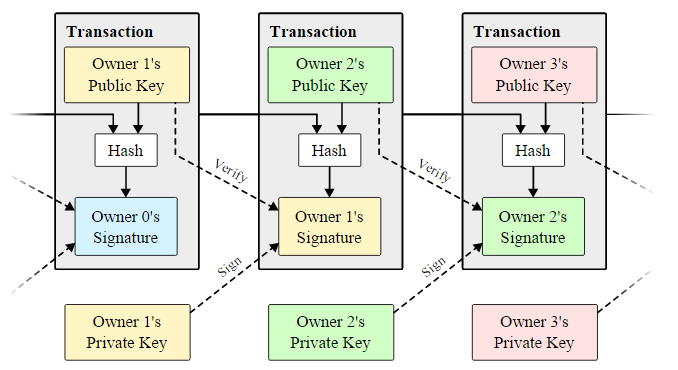
\includegraphics[width=\linewidth]{blockchaintransactions.png}
 	\caption{Voorbeeld van transacties. Bron: Bitcoin.org/bitcoin.pdf}
 	\label{fig:blockchain-transaction-example}
 \end{figure}
\begin{figure}
	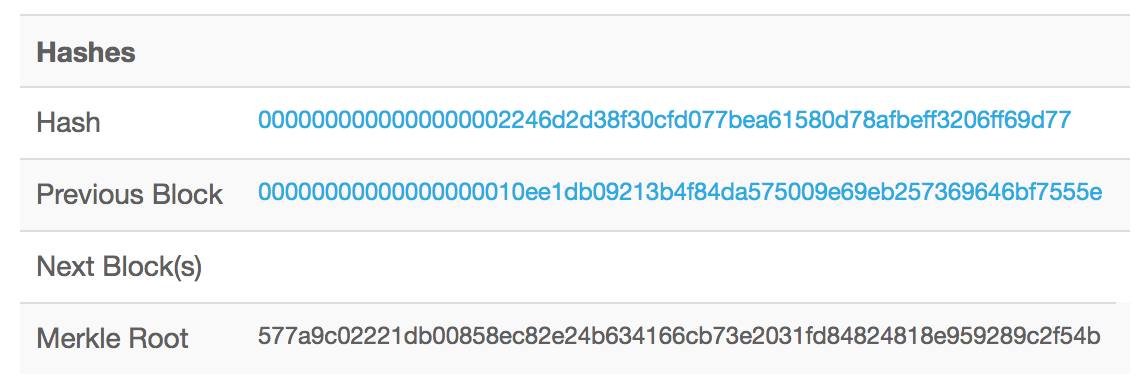
\includegraphics[width=\linewidth]{blockchain-hashes.png}
	\caption{Voorbeeld van hashes. Bron: https://blockchain.info/}
	\label{fig:blockchain-hash-example}
\end{figure}
 
 \subsubsection{Initaliseren van een blockchain}
 Natuurlijk moet er wel een manier zijn om bijvoorbeeld nieuw geld in de blockchain toe te voegen, dit moet dan uiteraard wel ergens vandaan komen dus er moet natuurlijk wel een manier zijn om instanties aan te kunnen maken. 
 
 De eerste transactie in een blok wordt gezien als een speciale transactie die meteen ook een nieuwe munt zal aanmaken waar hij eigenaar van is. Dus voor elke eerste transactie van een blok wordt een nieuwe munt aangemaakt waarvan de node dus eigenaar is. Dit zorgt meteen ook voor een goed motief om het netwerk van nodes te steunen en zorgt ook meteen voor een manier om nieuwe munten in omloop te brengen aangezien er geen centrale authoriteit is die de blockchain beheert. 
 
 Er wordt dus constant geld toegevoegd aan de bitcoin blockchain door het gevolg van het verbruiken van middelen. In het geval van Bitcoin is dit bijvoorbeeld elektriciteit en CPU-kracht en dit zal voor de meeste blockchains ook het geval zijn. Dus met andere woorden wordt het openstellen van CPU-kracht en het gebruik hiervan beloond door het verkrijgen van bitcoins bij het aanmaken van een nieuw blok. Dit heeft ook als voordeel dat het proberen hacken van de blockchain niet meer zo gunstig zou zijn en het dus beter is om een ``eerlijke'' node te blijven. Natuurlijk is het niet nodig om steeds een nieuwe munt aan te maken als motivatie want dit zou zorgen voor inflaties. Wanneer er bijvoorbeeld een genoeg aantal munten in omloop zijn kan het gehele systeem van verbruikte middelen ook vergoed worden door transactiekosten zodat er helemaal geen inflatie optreed.
 
 \subsubsection{Kan iedereen zich aansluiten bij de nodes?}
 Iedereen kan inderdaad lid worden van een blockchain netwerk en CPU-kracht beschikbaar stellen, dit wordt ook ``gold miners'' genoemd. Je stelt je eigen computer ter beschikking als node in het netwerk waardoor jij vergoed wordt met bitcoins. Deze zouden dan ook de kosten moeten dekken van de elektriciteit en de verbruikte CPU-kracht. Wie dus CPU-kracht over heeft kan deze ter beschikking stellen en hier aan verdienen. Op deze manier probeert  bitcoin bijvoorbeeld ook om alle nodes ``eerlijk'' te houden aangezien dit veel interessanter zou zijn. Het opstellen van een gold miner wordt later uitgelegd. 
 
 Tegenwoordig kan je niet meer je eigen computer ter beschikking stellen voor Bitcoin aangezien de verloning voor elektriciteit en CPU-kracht te laag zou zijn om dit competetief te houden. Daarom is er tegenwoordig hardware te koop om Bitcoins te minen die gemaakt zijn speciaal hiervoor. Deze zijn meteen ook veel zuiniger. Dit volgens het volgende artikel \textcite{Bitcoinmining.com}.
 
 \subsubsection{Hoe gebeurd de validatie?}
 Hoe wordt er voorkomen dat er illegale transacties worden uitgevoerd? Het hele systeem werkt aan de hand van peer-to-peer, elke server heeft dus zijn eigen versie. Telkens er een verandering wordt uitgevoerd dan wordt de blockchain verandering gebroadcast over het hele netwerk. Vervolgens gaat elke node die de transactie ontving deze gaan plaatsen in een blok. Elke node zal vervolgens een moeilijke proof-of-work genereren. Wat een proof-of-work juist is wordt uitgelegd in volgend puntje. Wanneer een node een proof-of-work gegenereerd heeft dan zal hij deze block versturen naar alle andere nodes in het netwerk. Vervolgens zullen de nodes het block enkel en alleen aanvaarden als alle transacties in het block kloppen en nog niet vervallen zijn. Om aan te tonen dat een node het block heeft aanvaard zal deze node de hash van deze block gebruiken in de volgende block als vorige hash. 

\begin{figure}
	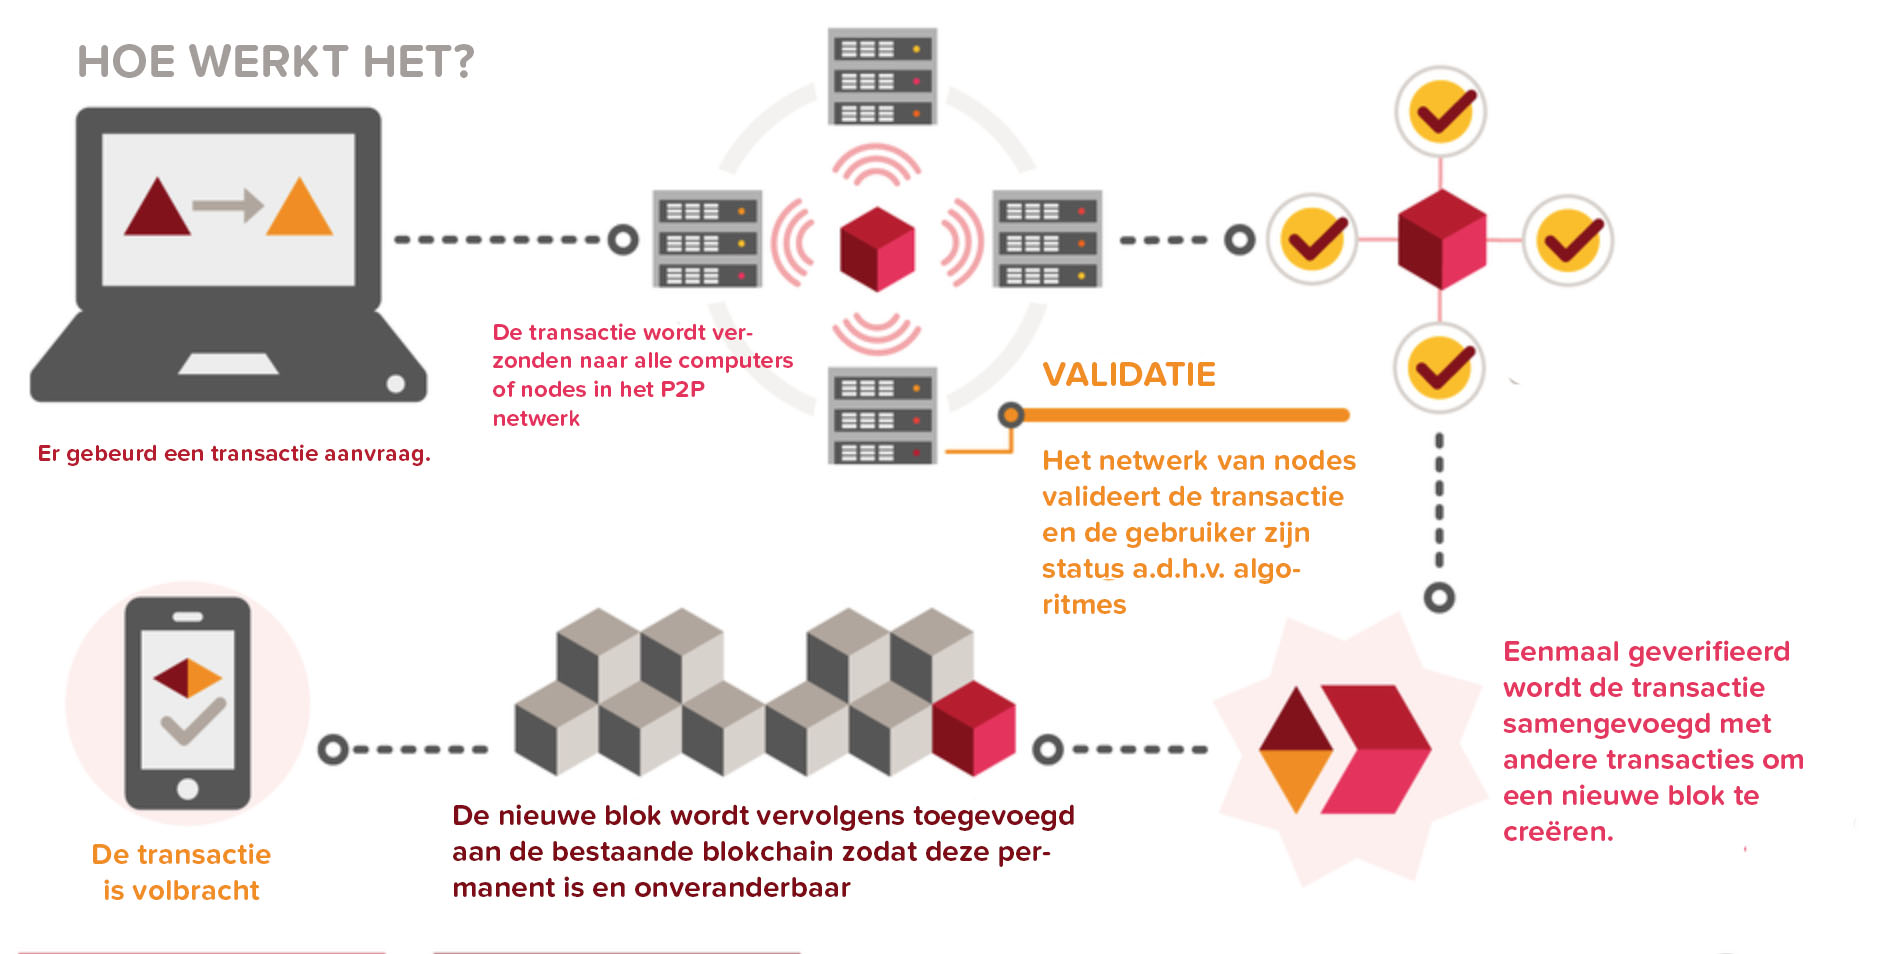
\includegraphics[width=\linewidth]{blockchain-howto.jpg}
	\caption{Grafische voorstelling van de werking van blockchain. Bron: http://usblogs.pwc.com/emerging-technology/wp-content/uploads/2016/11/blockchain-infographic.0.png}
	\label{fig:blockchain-howto}
\end{figure}

In het algemeen zullen de nodes altijd de langste ``ketting'' aanvaarden als de correcte en zal het verder werken aan deze ketting. Wanneer twee nodes een verschillend blok gaan broadcasten dan kan het zijn dat één node de ene versie eerst zal krijgen en een andere de alternatieve versie eerst zal ontvangen. Daarom zal altijd de eerste die ontvangen werd gebruikt worden. De alternatieve versie wordt dan bijgehouden. Deze koppeling wordt onderbroken vanaf er een nieuwe proof-of-work wordt gevonden. Hierdoor zal één van de twee versies langer worden en de langste versie zal dan gebruikt worden om op verder te bouwen. De nodes die ondertussen op de andere tak aan het werken waren zullen dan ook overschakelen op deze. Dit wil natuurlijk niet zeggen dat een transactie broadcast alle nodes moeten bereiken, het blijft steeds het internet en een transactie kan verloren geraken. Dit is geen probleem zolang er maar genoeg nodes de transactie ontvangen en deze verifiëren. De nodes die die transactie niet ontvingen zullen dit merken wanneer ze de volgende blok ontvangen en zien dat ze er één hebben gemist en zal deze dan aanvragen aan de andere nodes in het netwerk. De volledige werking is visueel weergegeven op Figuur \ref{fig:blockchain-howto}

\subsubsection{Soorten in blockchain}

\begin{figure}
	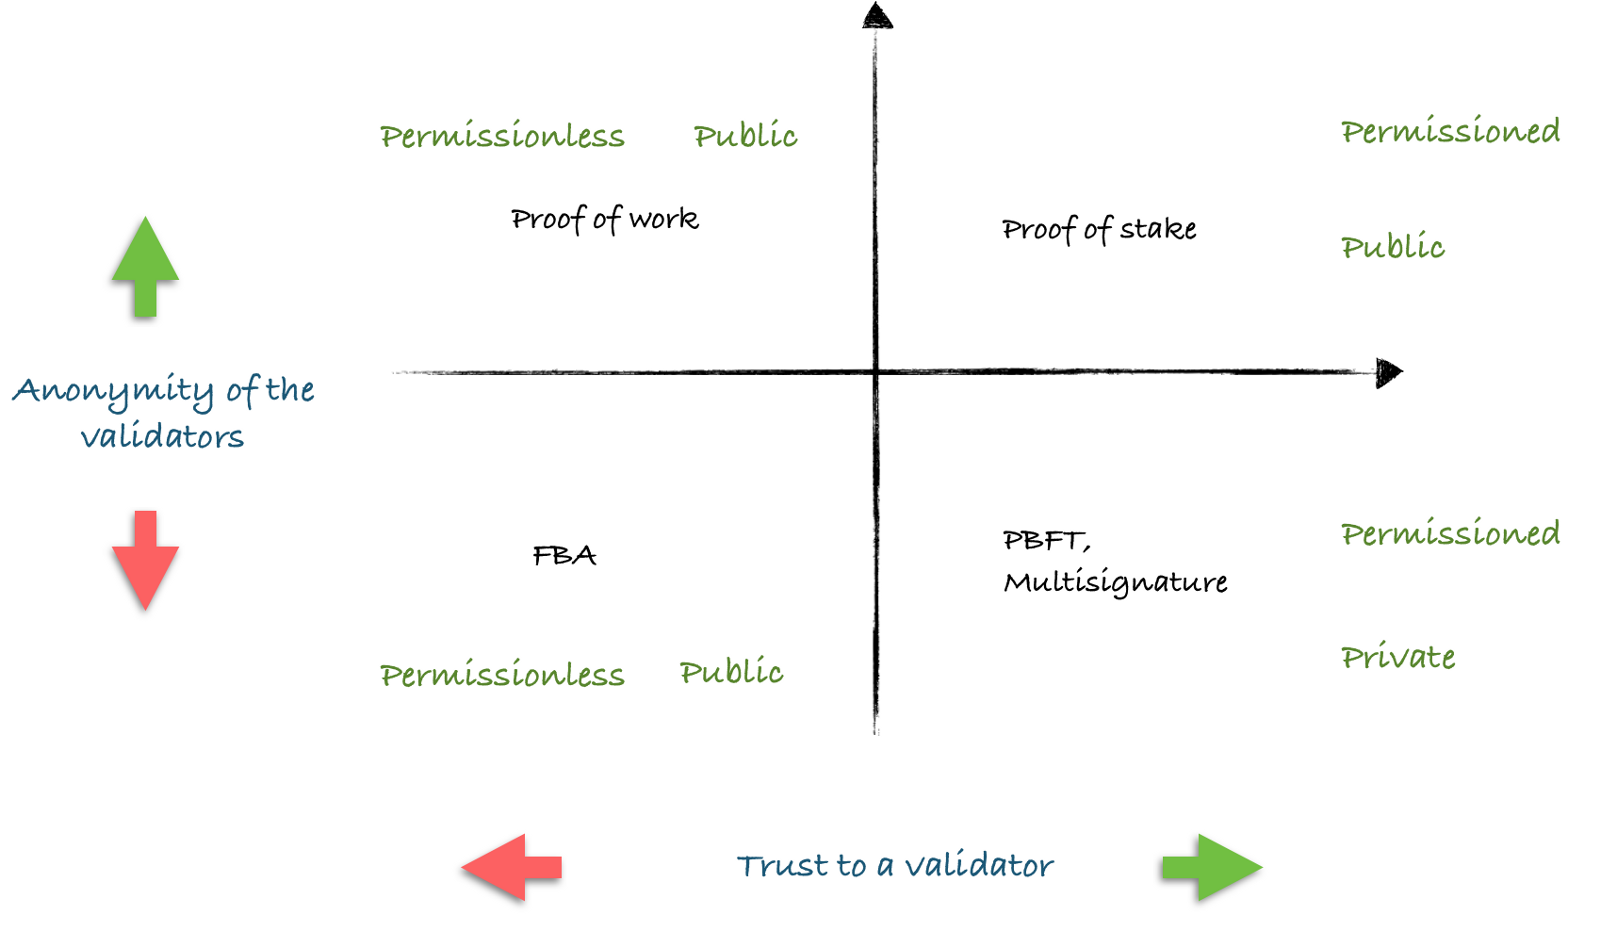
\includegraphics[width=\linewidth]{blockchain-types.png}
	\caption{Grafische voorstelling van enkele varianten van de blockchain types die bestaan. Enderzijds publieke versus private en anderzijds met rechten of zonder rechten. Bron: \textcite{Kravchenko2016}}
	\label{fig:blockchain-types}
\end{figure}

Natuurlijk zijn er verschillende soorten blockchain. Doorheen de literatuurstudie word telkens Bitcoin als voorbeeld gebruikt, Bitcoin is uiteraard een publiek netwerk waar geen rechten op toegekend waren. Dit volgens \textcite{Nakamoto2008}. Natuurlijk is dit niet de enige soort en zijn er nog andere varianten die telkens toch wat verschillen hebben. Hoofdzakelijk zijn er 2 veranderlijken, de anonimiteit en de hoeveelheid vertrouwen die de gebruiker heeft. \textcite{Kravchenko2016} maakte hierover een uitgebreid artikel en gebruikte het volgende schema dat te zien is op Figuur \ref{fig:blockchain-types}.

Wie zien meteen dat Blockchain bovenaan links in de groep hoort. Niemand is gekend op het netwerk, er zijn geen rechten van toepassing en iedereen heeft toegang. De enige manier van validatie die hier van toepassing is, is proof-of-work. Je moet dus nooit op voorhand hebben deelgenomen of doorgelicht geweest zijn om deel te kunnen nemen. Het vertrouwen dat aan een ``miner'' wordt gegeven is laag en er is ook geen straf voor het aanvallen van het systeem buiten het feit dat de mining apparatuur niet verder kan gebruikt worden als de aanval succesvol was. Dit type is dus vooral geschikt voor volledig anonieme systemen die volledig buiten een overheidinstanties werken. 

Bovenaan rechts is een publieke blockchain maar deze keer wel met rechten. Dit omdat er munten moeten gekocht worden om te kunnen minen. Een munt is dan ook iets wat van het systeel zelf is en niet werkt zoals Bitcoin waar een munt wordt gegeven aan de eigenaar van mining machines. Deze soort beveiliging wordt ook ``proof of stake'' genoemd. Dit soort systemen geven hierdoor ook meer vertrouwen aan de gebruiker aangezien bij een aanval op het syteem de ``borg'' verloren gaat bij het proberen uitvoeren van een aanval of dubbele uitgave. Dit soort systemen is ideaal voor de uitvoering van contracten, gemeenschapsbestuur, privé geld systemen, enz. 

Onderaan links vinden we de privé blockchain zonder regels. Onder bepaalde sociale overeenkomsten kan iedereen toegang krijgen tot het syteem en dus een node worden in het systeem. Een goed voorbeeld hiervan is bijvoorbeeld een land waar elke bewoner toegang heeft om een node te worden van het netwerk. Het vertrouwen dat wordt gegeven aan een node is vrij laag, zelfs met de identiteit die gekend is. Dit is meteen ook een groot verschil met de bitcoin variant waar iedereen niet gekend is. Hoe komen systemen dan overeen bij validatie van data? In praktijk toont dat een FBA (Federated Byzantine Agreement) overeenkomst het beste is in de meeste gevallen. Proof of stake kan hier bijvoorbeeld niet gebruikt worden aangezien elke node evenveel inspraak heeft. Dit zou bijvoorbeeld goed werken voor nationale blockchains en dergelijke. 

Als laatste hebben we nog het kwadrant dat onderaan rechts ligt. Dit kwadrant bevat de blockchain die volledig afgeschermd is, dus volledige privé en met regels. Om te kunnen deelnemen moet men dus een soort licentie hebben of deel zijn van een groep. Deze soort van blockchain is vooral bruikbaar in bedrijven, banken en andere zaken. Overeenkomst tussen de systemen kan snel gebeuren aangezien er veel vertrouwen wordt gegeven aan de nodes, een aanval op het systeem zorgt dan ook meteen voor het verliezen van de licentie en dus toegang of het verwijderd worden uit de groep. Als validatie overeenkomst tussen de nodes wordt PBFT of multisignature gebruikt. Een groot voordeel zoals eerder vermeld is het snel afhandelen van overenkomsten. 

\subsubsection{Wat betekent proof-of-work?}
Proof-of-work is een maatregel die werd ingevoerd om bepaalde aanvallen te voorkomen zoals de gekende denial of service of ook DOS-aanvallen genoemd of om spam op een netwerk tegen te gaan en dit door werk te vragen van de service aanvrager meestal in de vorm van verwerkingstijd door een computer. Proof-of-work kan voorkomen in verschillende vormen, meestal zijn dit wiskundige algoritmen. Enkele voorbeelden zijn puzzels, Diffie-Hellman puzzels, hash sequencies, Merkle tree gebaseerde algoritmen en nog enkele meer. 

Verder zijn er ook verschillende varianten. Deze zijn de Challenge-response en Solution-verification. Het verschil tussen beide kort samengevat komt neer op het volgende, bij challenge-response is de taak die moet uitgevoerd worden nog niet bekend. De server zal deze sturen bij het aanvragen van een service. Bij Solution-verification is de taak op voorhand gekend en kan deze meteen meegestuurd worden met de request. Deze informatie is terug te vinden op  \textcite{Wikipedia-POW}. Een grafische voorstelling van beide is te vinden op Figuur \ref{fig:pow-challengeresponse} en Figuur \ref{fig:pow-solutionverification}. De proof-of-work die Bitcoin zelf gebruikt is bijvoorbeeld gebaseerd op Adam Back's Hashcash, dit volgens \textcite{Nakamoto2008}.

Verder is er nog een soort systeem dat ook als blockchain beschouwd wordt, multi-blockchain systemen. Dit is een set van protocols dat nodes toelaat om een gepast consensus mechanisme te gebruiken. 

\begin{figure}
	
\includegraphics[width=\linewidth]{pow-challengeresponse.png}
	\caption{Grafische voorstelling van de werking van challenge response. Bron: en.wikipedia.org/wiki/Proof-of-work\_system}
	\label{fig:pow-challengeresponse}
\end{figure}

\begin{figure}
	
\includegraphics[width=\linewidth]{pow-soultionverification.png}
	\caption{Grafische voorstelling van de werking van solution verification. Bron: en.wikipedia.org/wiki/Proof-of-work\_system}
	\label{fig:pow-solutionverification}
\end{figure}

\subsubsection{Hoe veilig is blockchain?}
\label{sec:hoeveiligisblockchain}
Wanneer er dus een aanval gebeurt op de blockchain of dus een illegale transactie plaats vindt dan kan deze verworpen worden door de andere servers. In simpele termen komt het er op neer dat zolang de totale CPU capaciteit van de servers groter is dan de capaciteit van de aanvaller dat de blockchain dus veilig is en de aanvallen zal afweren. Dit omdat de aanvaller sneller een alternatieve ketting zou moeten produceren  dan dat de vertrouwde nodes dit doen. Zelf in het geval dat dit zou gebeuren wil dit niet zeggen dat de vertrouwde nodes dit zullen accepteren aangezien dat de aanvaller ook geen waarde kan creëren uit het niets of zichzelf eigenaar kan maken van andere waarden als we dit zouden bekijken in het systeem van Bitcoins. Het enige wat een aanvaller dus in principe kan doen is het aanpassen van zijn eigen transacties, bijvoorbeeld dus geld terug nemen dat hij al eerder uitgaf of ook ``double spending'' genoemd. Verder zijn er natuurlijk nog andere mogelijkheden waar er rekening moet mee gehouden worden op vlak van veiligheid, meer hierover in de volgende paragraaf. De kans dat zich dit voordoet is uitermate klein. Zo is te zien in de whitepaper van \textcite{Nakamoto2008}. Stel dat de aanvaller 10 blokken achter zit en de vertrouwde ketting moet inhalen dan heeft deze een kans van 0.0000012\% wanneer we er vanuit gaan dat de aanvaller 10 \% kans heeft om de volgende blok te vinden. Verdere berekeningen zijn te vinden in de paper van \autocite{Nakamoto2008}.


\subsubsection{Andere soorten ``hacks''}
Er zijn uiteraard verschillende manieren van ``hacken'', één van de bekendste is bitcoin mining malware. Dit is malware die verspreid wordt en computers en apparaten infecteerd. De geïnfecteerde apparaten worden hierdoor gebruikt om bitcoins te minen wat de toestellen uiteraard zwaar vertragen. 

Andere zaken die veel voorkomen zijn het hacken van de bitcoin wallets, dit zijn bestanden die op de machine staan en die de bitcoins bij houd. Deze ``wallets'' bevinden zich op de hardeschijf en kunnen dus gestolen worden. 

Trojans zijn ook bij bitcoin een plaag. Zo zijn er trojans die slechts activeren wanneer er een crypto-currency nummer wordt ontvangen en die deze dan manipuleren zodat de gebruiker bijvoorbeeld geld overschrijft naar de verkeerde persoon. 

Verder zijn er ook nog fouten in de software die bijvoorbeeld toegang geeft tot een blockchain. Blockchain mag in theorie en praktijk nog zo veilig zijn, als er software gebruikt wordt die malfunctioneert dan kan de veiligheid van blockchain ook snel te niet gedaan worden.

Zoals eerder vermeld zijn de transacties of sommige zaken versleuteld voor het publiek. De transactie zelf is zichtbaar maar sommige zaken zijn versleuteld. Wanneer deze encryptie bijvoorbeeld niet sterk genoeg is kan het zijn dat hackers een bepaald deel van de versleutelde tekst toch kan ontfutselen. Blockchain gebruikt in het algemeen een SHA-256 versleuteling, deze word onder andere ook gebruikt voor het versleutelen van HTTPS en dergelijke. Wanneer deze encryptie zou falen zou niet enkel blockchain dus een zwaar probleem hebben. Onderzoekers bevestigden wel dat SHA-256 zeker sterk genoeg is om zaken te beveiligen voor een hele tijd.

\subsubsection{Wat is SHA-256}
SHA-2 is een verzameling van cryptografische hash functies die gemaakt werden door de National Security Agency (NSA). Wat zijn cryptografische hash functies? Dit zijn wiskundige bewerkingen die kunnen uitgevoerd worden op digitale data. Door vervolgens de berekende ``hash'' te vergelijken met de verwachte hash kan men de data integriteit bepalen. Dit volgens volgend artikel \textcite{Wikipedia-Sha} Om een voorbeeld te geven om dit principe te verduidelijken nemen we het volgende voorbeeld. We hebben een bestand gedownload, laat ons zeggen dat dit een ``word'' bestand is. We maken een kopie van dit bestand en passen in het word document enkele dingen aan. We slaan vervolgens het document op en berekenen de hash van beide documenten. Nu hebben we dus het originele bestand en het aangepaste bestand. Als we nu de hash zouden vergelijken van beide documenten dan gaan we zien dat deze verschillen. Mochten we nu van de originele versie nog een kopie maken en hiervan de hash berekenen dan zal deze dezelfde zijn van het originele bestand. Op deze manier kunnen we dus bekijken of een bestand gewijzigd is of niet. Een grafisch voorbeeld van dit voorbeeld is te zien in Figuur \ref{fig:hash-example}.

 \begin{figure}
 	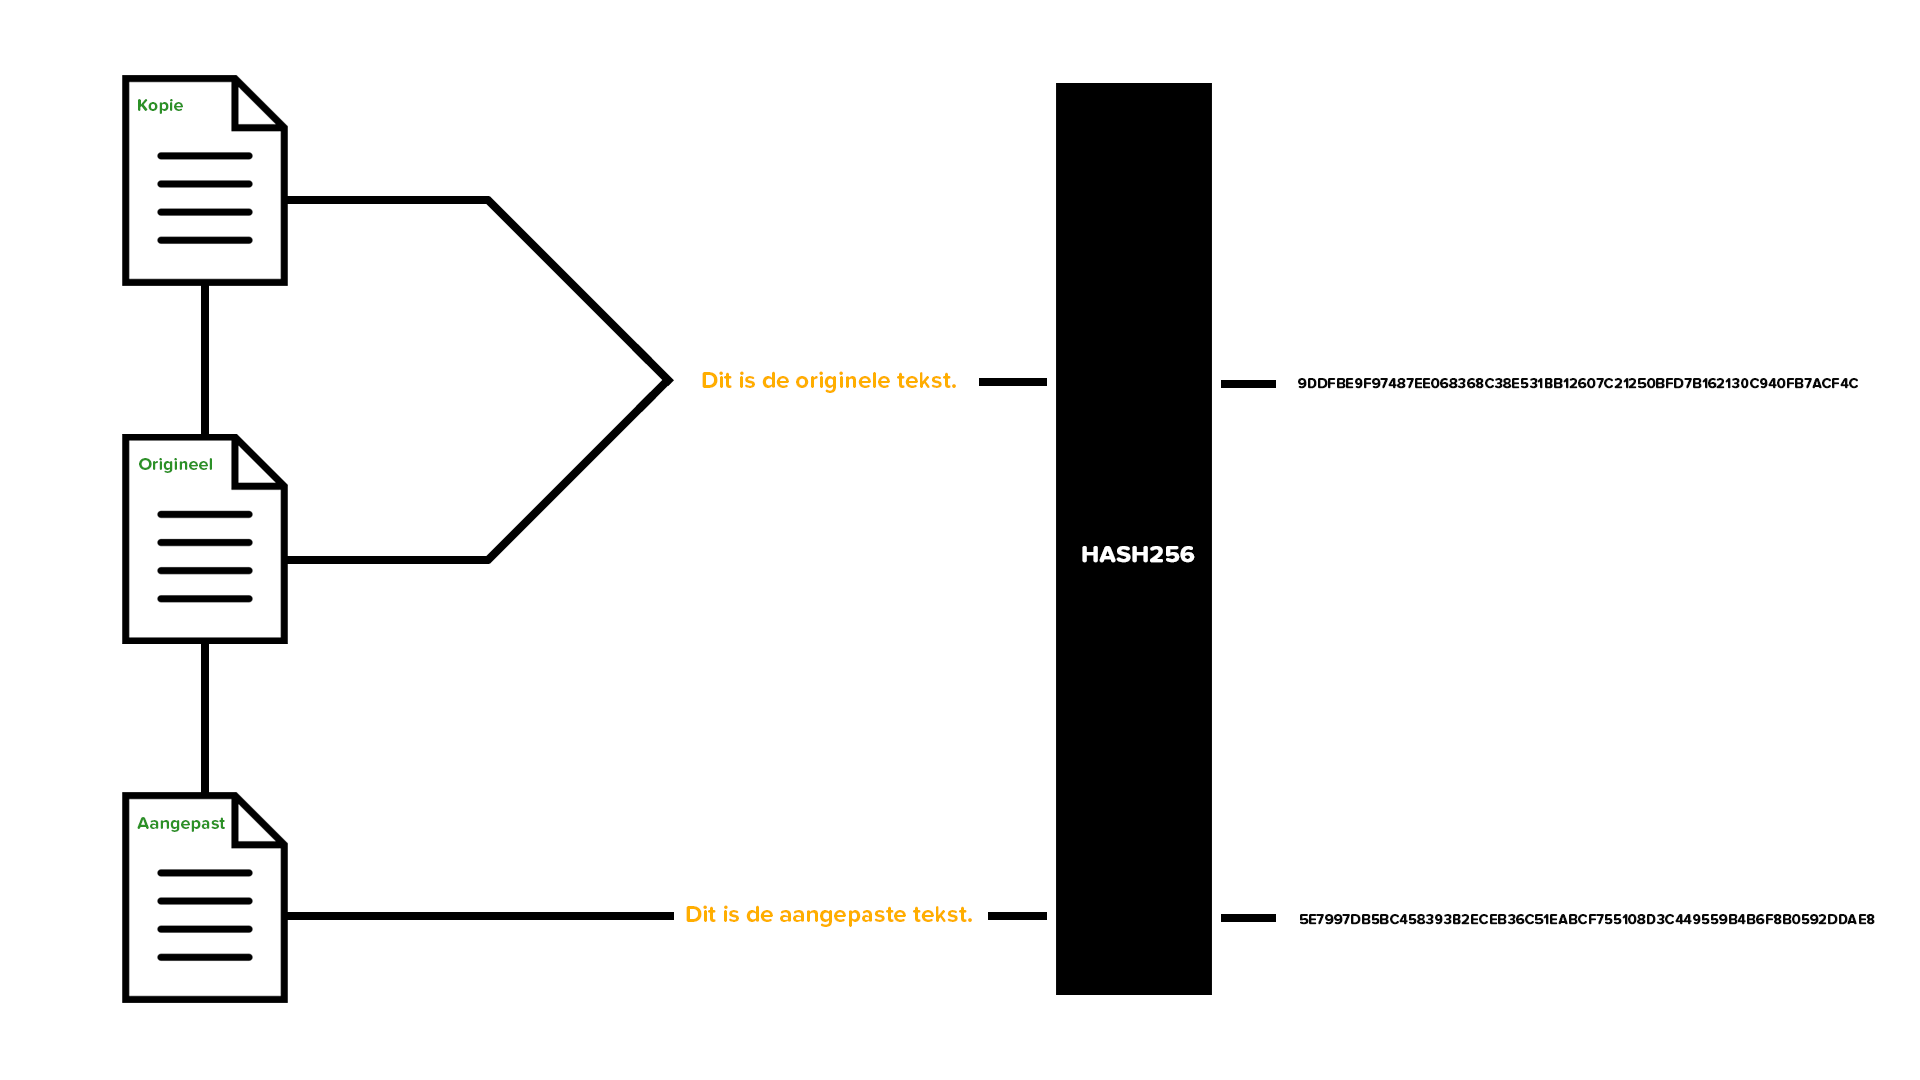
\includegraphics[width=\linewidth]{hash-example.png}
 	\caption{Grafische voorstelling van de werking van sha256.}
 	\label{fig:hash-example}
 \end{figure}



\subsection{Verzekeringen en unieke documenten}
\subsubsection{Wat is een verzekeringsagent en een verzekeringsmakelaar?}
Een verzekeringsagent is een gebonden tussenpersoon. Dit wil zeggen dat deze persoon voor één verzekeringsmaatschapij werkt, dit verschillend van een verzekeringsmakelaar die onafhankelijk is en niet gebonden is aan één verzekeringsmaatschapij. Een verzekeringsagent kan dus slechts de verzekeringen aanbieden van zijn eigen maatschapij waar een verzekeringsmakelaar verzekeringen kan aanbieden van verschillende maatschapijen. 

Er zijn uiteraard meerdere benamingen voor een verzekeringsagent die allemaal op hetzelfde neerkomen zo wordt een verzekeringsagent bijvoorbeeld ook een tussenpersoon genoemd, een intermediair of een financieel adviseur. 

\subsubsection{Wat doet een verzekeringsagent of verzekeringsmakelaar?}
Zoals eerder vermeld doet een verzekeringsagent en verzekeringsmakelaar juist hetzelfde. Het enige verschil tussen beide is dus dat een verzekeringsagent gebonden is aan één maatschapij waar een verzekeringsmakelaar dit niet is. Voor vereenvoudiging doorheen dit document zal ik steeds verwijzen naar een verzekeringsmakelaar. 

Wat doet een verzekeringsmakelaar nu juist? Een verzekeringsmakelaar zal jouw wensen en vragen allemaal noteren en zal dit gebruiken om de voor u zo optimale verzekering te vinden. Nadien overloopt deze dan alle mogelijkheden met de nodige uitleg. Verzekeren kan een zeer complex iets zijn en dan is een verzekeringsmakelaar zeker nuttig om te raadplegen. Dit alles is te vinden in volgend document \textcite{Verzekeruzelf.nl}.

\subsubsection{Soorten verzekeringen en verzekeringsdocumenten}
Er zijn heel veel soorten verzekeringen. Zo kan in theorie alles verzekerd worden al is dit niet altijd gebruikelijk. In volgend document \textcite{verzekeringen.com2015} vind je alvast enkele voorbeelden van beroemdheden die verschillende lichaamsdelen lieten verzekeren want ook dit is uiteraard mogelijk. Bijvoorbeeld wanneer een gitarist zijn hand zou verliezen dan verliest deze hiermee ook meteen de mogelijkheid tot het uitoefenen van zijn beroep. Er zijn dus heel wat mogelijkheden beschikbaar, volgens het volgende artikel \textcite{BFOverzekeringen} van de Belgische overheid zijn dit de meest voorkomende verzekeringen.

\begin{itemize}
	\item Autoverzekering
	\item Brandverzekering en natuurrampen
	\item Familiale BA-verzekering
	\item Rechtsbijstand
	\item Ziekte- en hospitalisatieverzekering
	\item Reisverzekering
	\item Vrijwilligersverzekering
	\item Schuldsaldoverzekering
	\item Levensverzekering of overlijdensverzekering
	\item Verzekeringen in specifieke situaties
\end{itemize}

Voor elk van bovenstaande verzekeringen is er dus een contract, dit bijgevolge ook uniek zal zijn en bepaalde voorwaarden zal bevatten. Documenten zoals deze zouden dus perfect in een blockchain kunnen opgeslagen kunnen worden. 

\subsubsection{Is verzekeren verplicht?}
Er wordt inderdaad ook onderscheid gemaakt tussen verplichte verzekeringen en niet verplichte verzekeringen. Zo kan je verplicht zijn een verzekering te nemen om een bepaalde activiteit te mogen uitvoeren. Denk maar aan een BA verzekering, wanneer je wagen niet verzekerd is dan kan deze niet in verkeer worden gebracht. Daar tegenover is een bestuurdersverzekering geen verplichte verzekering. Ook voor het uitvoeren van bepaalde beroepen is het verplicht om een verzekering aan te gaan. Enkele voorbeelden zijn architecten, boekhouders, belastingsconsulenten en nog vele meer. Sommige verzekeringen kunnen dan weer wel contractueel verplicht worden. Zo kan een huisbaas bijvoorbeeld de huurder verplichten een brandverzekering af te sluiten. Dit volgens het volgende artikel van \textcite{BFOverplichteVerzekeringen}. 

%%\lipsum[7-20]

\section{Probleemstelling en Onderzoeksvragen}
\label{sec:onderzoeksvragen}

%% TODO:
%% Uit je probleemstelling moet duidelijk zijn dat je onderzoek een meerwaarde
%% heeft voor een concrete doelgroep (bv. een bedrijf).
%%
%% Wees zo concreet mogelijk bij het formuleren van je
%% onderzoeksvra(a)g(en). Een onderzoeksvraag is trouwens iets waar nog
%% niemand op dit moment een antwoord heeft (voor zover je kan nagaan).

\section{Opzet van deze bachelorproef}
\label{sec:opzet-bachelorproef}

%% TODO: Het is gebruikelijk aan het einde van de inleiding een overzicht te
%% geven van de opbouw van de rest van de tekst. Deze sectie bevat al een aanzet
%% die je kan aanvullen/aanpassen in functie van je eigen tekst.

De rest van deze bachelorproef is als volgt opgebouwd:

In Hoofdstuk~\ref{ch:methodologie} wordt de methodologie toegelicht en worden de gebruikte onderzoekstechnieken besproken om een antwoord te kunnen formuleren op de onderzoeksvragen.

%% TODO: Vul hier aan voor je eigen hoofstukken, één of twee zinnen per hoofdstuk

In Hoofdstuk~\ref{ch:conclusie}, tenslotte, wordt de conclusie gegeven en een antwoord geformuleerd op de onderzoeksvragen. Daarbij wordt ook een aanzet gegeven voor toekomstig onderzoek binnen dit domein.


%%=============================================================================
%% Methodologie
%%=============================================================================

\chapter{Methodologie}
\label{ch:methodologie}

%% TODO: Hoe ben je te werk gegaan? Verdeel je onderzoek in grote fasen, en
%% licht in elke fase toe welke stappen je gevolgd hebt. Verantwoord waarom je
%% op deze manier te werk gegaan bent. Je moet kunnen aantonen dat je de best
%% mogelijke manier toegepast hebt om een antwoord te vinden op de
%% onderzoeksvraag.

\lipsum[21-25]



%% Voeg hier je eigen hoofdstukken toe die de ``corpus'' van je bachelorproef
%% vormen. De structuur en titels hangen af van je eigen onderzoek. Je kan bv.
%% elke fase in je onderzoek in een apart hoofdstuk bespreken.

%\input{}
%\input{}
%...

%%=============================================================================
%% Conclusie
%%=============================================================================

\chapter{Conclusie}
\label{ch:conclusie}

%% TODO: Trek een duidelijke conclusie, in de vorm van een antwoord op de
%% onderzoeksvra(a)g(en). Wat was jouw bijdrage aan het onderzoeksdomein en
%% hoe biedt dit meerwaarde aan het vakgebied/doelgroep? Reflecteer kritisch
%% over het resultaat. Had je deze uitkomst verwacht? Zijn er zaken die nog
%% niet duidelijk zijn? Heeft het onderzoek geleid tot nieuwe vragen die
%% uitnodigen tot verder onderzoek?

\lipsum[76-80]


\appendix

%%---------- Back matter ------------------------------------------------------

\printbibliography
\addcontentsline{toc}{chapter}{\textcolor{maincolor}{\IfLanguageName{dutch}{Bibliografie}{Bibliography}}}


\listoffigures
\listoftables

\end{document}
